\documentclass[a4paper,8pt,openany]{book}
\usepackage [utf8]{inputenc}
\usepackage [french]{babel}
\usepackage [T1]{fontenc}
\usepackage{listings}
\usepackage{graphicx}
\usepackage{verbatim}
 \usepackage{amsmath} 

%%configuration de listings
\lstset{
language=c,
basicstyle=\ttfamily\small, 
identifierstyle=\color{red}, 
keywordstyle=\color{blue}, 
stringstyle=\color{black!60}, 
commentstyle=\it\color{green!95!yellow!1}, 
columns=flexible, 
tabsize=1, 
extendedchars=true, 
showspaces=false, 
showstringspaces=false, 
numbers=left, 
numberstyle=\tiny, 
breaklines=true, 
breakautoindent=true, 
captionpos=b
}

%coloration syntaxique
\usepackage{xcolor}
\definecolor{Zgris}{rgb}{0.87,0.85,0.85}

\newsavebox{\BBbox}
\newenvironment{DDbox}[1]{
\begin{lrbox}{\BBbox}\begin{minipage}{\linewidth}}
{\end{minipage}\end{lrbox}\noindent\colorbox{Zgris}{\\usebox{\BBbox}}
[.5cm]}

%Pour l espace entre la section et la chapitre (qui est trop grand).
\usepackage{titlesec}

\titleformat{\chapter}[block]
  {\normalfont\Huge\bfseries}% font of number
  {\chaptertitlename\ \thechapter~:}% format of number
  {20pt}% space between number and title
  {\Huge}% font of title

\titlespacing*{\chapter}
  {0pt}%  indent
  {0pt}% space before
  {20pt}% space after
\titlespacing*{\section}
  {0pt}%  indent
  {3.5ex plus 1ex minus .2ex}% space before
  {2.3ex plus .2ex}% space after

\author{Mendy Fatnassi}
\title{Cours Codage de l'information}

%%%%%%%%%%%%%%%%%%%%%%%%%%%%%%%%%%%%%%	Page	%%%%%%%%%%%%%%%%%%%%%%%%%%%%%%%%%%%%%%%%
\begin{document}
\maketitle
\tableofcontents

\chapter{Codage Physique / Codage sans perte}
\section{Introduction}

C'est en 1948 grace aux travaux de shannon , que la theorie de l'information a pris sa forme actuelle.\\
Le traitementdu contenue d'une source d'information peux etre envisage sous deux forme :\\
-Sans perte d'information.\\
-Avec perte d'information.\\
\\
\section{Transmissions Avec/Sans perte}
\textbf{Avec perte} : \\
\underline{Exemple} : Signal analogique stereo , bande de frequence 0 a 20 Khz , echantillonnage 44,1Khz , 
quantification de 16b.\\
Donc $44.1\times 10+3\times 16\times 2=1.411$ MBits/sec\\
Ex MP3 : reduction a 128 Kbits/sec avec un taux de compression de 11.\\
\\
\textbf{Taux de compression} : \\
-Elimination des composantes spectrales.\\
-Utilisation du codage de Huffman.\\
\\ 
La transmission numerique passe par un support physique qui interprete la communication sous forme de signaux numerique.Ainsi des donnees analogique devront prealablement erte numerise.Le codage du signaux peux se faire sur 2 (-X,X) ou 3 niveaux (-X,0,X).\\ 
\\

\section{Mode de transmission/Codage}
Voici quelque mode de transmission :\\
\\

\subsection{NRZ (No Return to Zero)}\\
\underline{Avantage}: Le recepteur peux determiner la presence ou non d'un signal.\\
\underline{Inconvenient} : Difficult\'e de synchronisation.\\
$0 \Rightarrow -X$\\
$1 \Rightarrow +X$\\
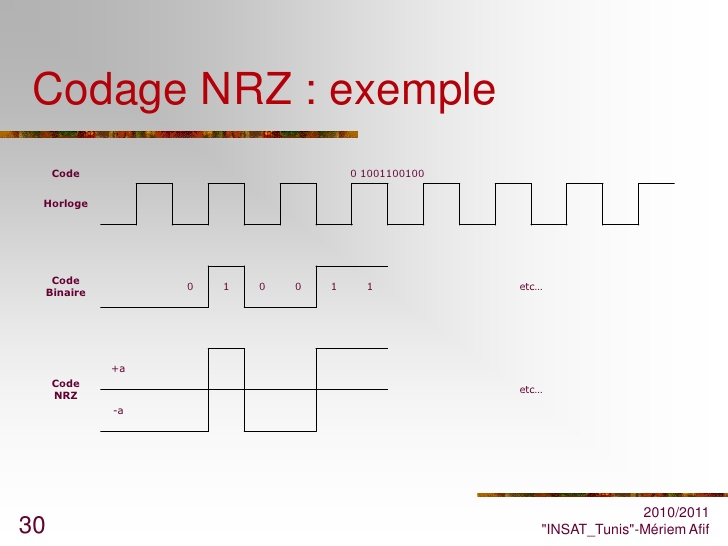
\includegraphics[width=0.75\textwidth,center]{img/nrz.jpg}\\
\\
Quelque derivée du NRZ : RZ(Return to Zero) \& NRZI (Inverted).\\ 
\subsubsection{RZ} : \\
pareil que pour NRZ sauf que entre deux bits 1 consecutif il y a un changement d'etat au lieu de reste sur +X on feras +X-X+X-X.\\
\\
\subsubsection{NRZI} : \\
1 $\Rightarrow$ le signal change d'etat , 0 $\Rightarrow$ aucun changement d'etat.\\
\\
\subsection{Unipolaire}\\
\underline{Avantage} : Reduction encore plus significative du spectre.\\
\underline{Inconvenient} : Impossibilite de distinguer une suite de 0 et l'absence d'information.\\
0 $\Rightarrow$ 0 (tension nulle)\\
1 $\Rightarrow$ +X\\ 
\\

\subsection{Bipolaire} : \\
0 $\Rightarrow$ lorsque le bit est a 0\\
1 $\Rightarrow$ alternativement +X et -X\\
\\
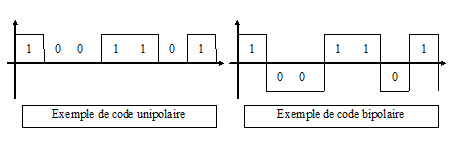
\includegraphics[width=1\linewidth]{img/code_uni_bipolaire.jpg}



\subsection{Manchester}\\
Une transition est introduite au milieu de l'intervalle significatif.\\
0 $\Rightarrow$ Transition du niveau bas vers le niveau haut ,front motant.\\
1 $\Rightarrow$ Transition di niveau haut vers le niveau bas , front descendant.\\
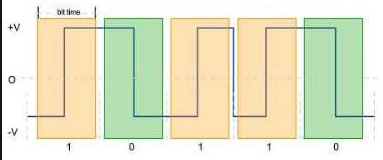
\includegraphics[width=1\linewidth]{img/code_manchester.png}
\\

\subsection{Delay Mode (Miller)}
Signal intermediaire identique au coodage manchester , puis suppression d'une transition sur deux.\\
Transition (front montant|descendant) $\Rightarrow$ 1\\
Pas de transition au milieu du bit 0\\
Transition en de fin de bit 0 si suivi d'un autre 0\\
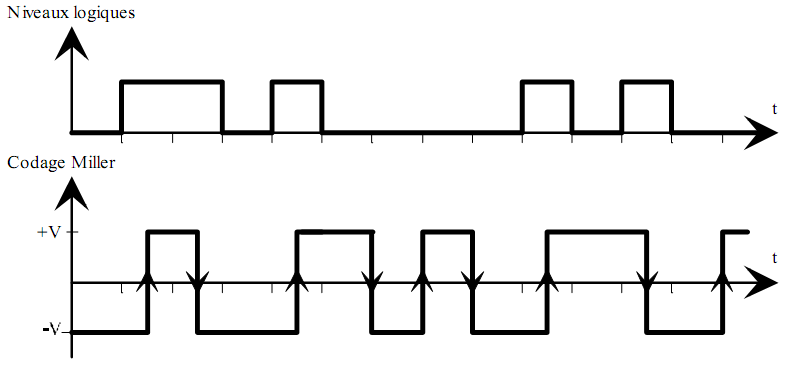
\includegraphics[width=1\linewidth]{img/code_miller.png}
\\



\subsection{HBDN} : \\
%%%%%%%%%%%%%%%%%%%A FAIRE%%%%%%%%%%%%%%%%%%%%%%%%%%%%ù

\section{Entropie}

La theorie de l'information men\'e par Shannon , qui est une théorie probabiliste permettant de quantifier le contenu moyen en information d'un ensemble de messages, dont le codage informatique satisfait une distribution statistique précise. Ce domaine trouve son origine scientifique avec Claude Shannon qui en est le père fondateur avec son article "A Mathematical Theory of Communication" publié en 1949.\\
Parmi les branches importantes de la théorie de l'information de Shannon, on peut citer :\\
-Le codage de l'information\\
-La mesure quantitative de redondance d'un texte\\
-La compression de données\\
-La cryptographie\\
\\
\underline{Paradigme de Shannon}:\\
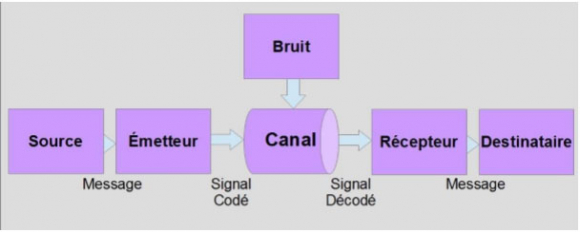
\includegraphics[width=0.75\linewidth,center]{img/modele_com_shannon.jpg}
\\
\textbf{L'entropie} permet de mesurer la quantit\'e d'information moyenne d'un ensemble d'\'venements (en particulier de messages) et de mesurer son incertitude.\\
Supposons maintenant que les boîtes soient de diverses couleurs : n1 boîtes de couleur C1, n2 boîtes de couleur C2…, nk boîtes de couleurs Ck, avec n1 + n2 + … + nk = N. La personne C sait de quelle couleur est la boîte recherchée. Quel est le prix de cette information ? .\\
On la note H(I) : $\sum_{i\in I} pi log_2 pi = -(p_i log p_i +...+ p_{i+n} log p_{i+n})$ \\
avec $pi=\frac{ni}{N}$ la probabilité associée à l'apparition de l'évènement i. \\
Donc l'information « la boîte est de couleur C1 » vaut log N/n1, et cette éventualité a une probabilité n1/N.\\
\\
Entropie d'une source discret (numerique:0,1) , si on a un message aleatoire avec un tirage de 27 lettres (alphabet + espace) , on aurait comme entropie H=log27=4,75 bits.\\
Entropie relative , elle dependra du contexte de son message (limit\'e par le corpus de la langue) et auras un pourcentage de libert\'e

\section{Codage Source}
Il existe des code a longueur fixe ou tous les mots ont la meme longueur et possede le meme nombre de symbole et les code a longueur variables ou la longueur varie en fonction de leur frequence d'apparition .Un mot sera d'autant plus long que sa probabilite d'apparition est  petite.\\

\subsection{Code de Shannon-Fano}
Deroulement de l'algo :\\
1-Trier les probabilit\'e par ordre descroissant\\
2-On separe l'ensemble en 2 groupes (de somme a peux pres egale)\\
3-$\sum1 = \sum2 \Rightarrow \sum1->0 \sum2->1$\\
4-On divise en 2 les deux sous-groupe $\sum1/2 = \sum11->0 , \sum21->1 $ et $ \sum2/2 = \sum21->0 , \sum22->1$\\
5-Bouclez de l'etape 4 a 5 jusqu'a tant de que le tableau soit remplie\\
\\
\underline{Exemple} : \\
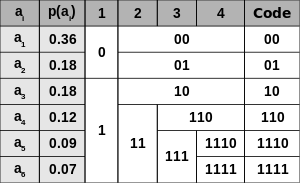
\includegraphics[width=0.75\linewidth]{img/code_shannon_fano.png}
\\
On a bien 2groupe qui ont des somme a peux pres egale avec a1,a2 > a3,a4,a5,a6 (0.54>0.46), la somme des a vaux bien 1.\\


\subsection{Code de Huffman}
Deroulement de l'algo :\\
1-Trier les probabilite par ordre croissant\\
2-creer un noeud parent a partir de 2 lettres sources avec les probabilite les plus faible\\
3-Affect\'e au noeud parent la somme des 2 noeud fils\\
4-Supprimer les noeud enfant\\
5-Bouclez de l'etape 2 a 5 jusqu'a ce que l'arbre soir remplie\\
\\
\underline{Exemple} : \\
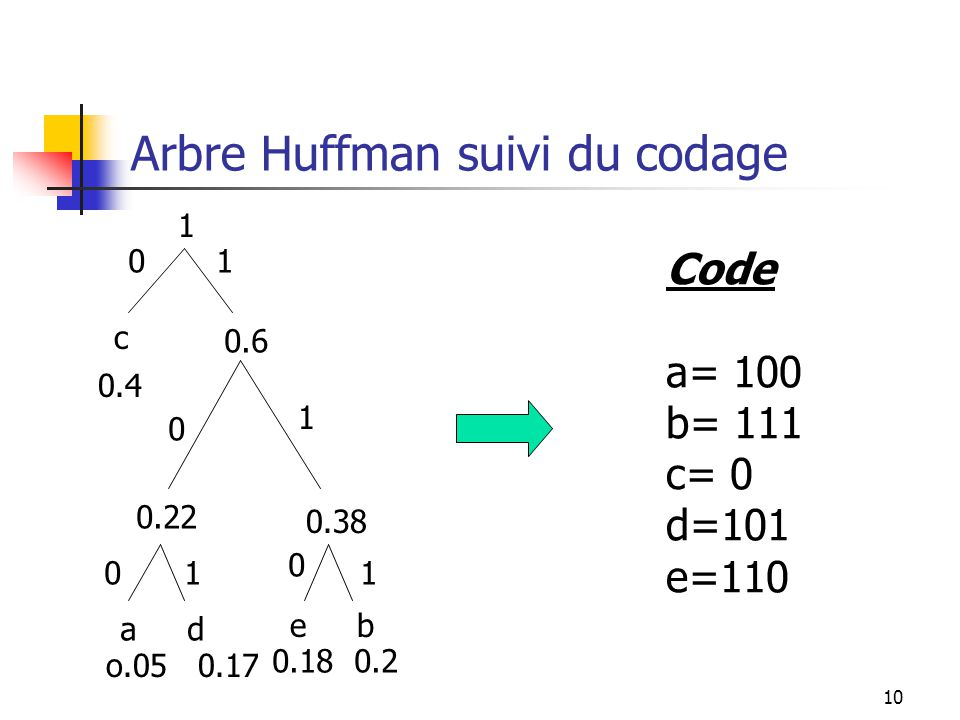
\includegraphics[width=1\linewidth]{img/code_de_huffman.jpg}
\\

\underline{Bonus} : Code LZW (Lempel-Ziv-Welch) utilis\'e  pour la compression des donn\'ees.\\

\subsection{Code Arithmetique}
%%%%%%%%%%%%%%%%%%%%%%%%%%%%%%%% a FAIRE%%%%%%%%%%%%%%%%%ù




%%%%%%%%%%%%%%%%%%%%%%%%%%%%%%%%%%%%%%%%%%%%%%%%%%%%%%%%%%%%%%%%%%%%%%%%%%%%%%
\chapter{Code Correcteur d'erreur / Code d'etalement}

\section{Introduction}
Un code correcteur d'erreur peux etre representer sous forme matriciel.Lors de la transmission numerique d'un signal il peux y avoir des causes d'erreur due a du bruit(thermique,impulsif,intermodulation,...),de la distortion,de l'echo ou du canal hertzien etc... .En general on ne peux agir sur le canal de transmission ou preferera se preoccuper sur le signal num. pour des contraintes tehchnologique et economique.\\
\\
On peux distinguer 2 types d'erreur :\\
-Les erreurs aleatoire due aux bruits blanc.\\
-Les erreurs par paquets (impulsif,parasite).\\
\\
\underline{Definition}\\
\textbf{bruit blanc} : On appelle la lumière blanche la superposition des ondes visibles du spectre. Et bien lorsqu’on superpose les fréquences audibles on obtient le bruit blanc. C’est un assemblage de plusieurs sons qui donnent un seul son uniforme.\\
\\
\section{Code Correcteur}
Il existe 2 type de code : \\
-Code en bloc\\
-Code convolutionnel\\
\\
Un code est appele $C(n,m)$ , la redondance est definie par : $\frac{m}{n}=1-\frac{k}{n} < 1$

\subsection{Code en Bloc}
Le message est decouper en bloc de $m eb(element binaire)$ de longueur fixe (m constant).A chaque bloc de $m eb$, le codeur ajoute $k eb$ de controle (appele checksum dans le cas du reseau) .On Vas ecrire $n=m+k$ , 
$n:m+k$ (n compos\'e de m+k) $\Rightarrow$ code s\'eparable ou syst\'ematique.\\

\subsection{Code Convolutionnel}
Des \'eb (echantillon binaire) de controle sont introduit de maniere continue dans le message utile .\'eb bloc : ajouter k eb de controle , depend du bloc de controle et anterieure $\Rightarrow$ code recurrent.\\

\section{Detection et Correction d'erreur}
Cas d'un canal sans symbole d'effacement.\\
\\
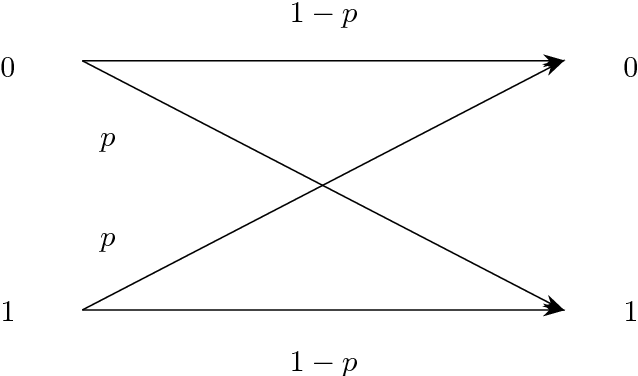
\includegraphics[width=0.5\linewidth]{img/sans_effacement.png}\\
\\
Code lineaire C de distance minimum $dm$ permet de :\\
-Detecter au plus $dm-1$ erreur\\
-Corriger au plus $t=\frac{dm-1}{2}$ erreur (entier)\\
\\
On dit qu'on code est lineaire systematique .(lineaire : informtion envoyee et messages recus , systematique : envoie bits de controle)\\
\\
Cas d'un canal avec symbole d'effacement : \\
\\
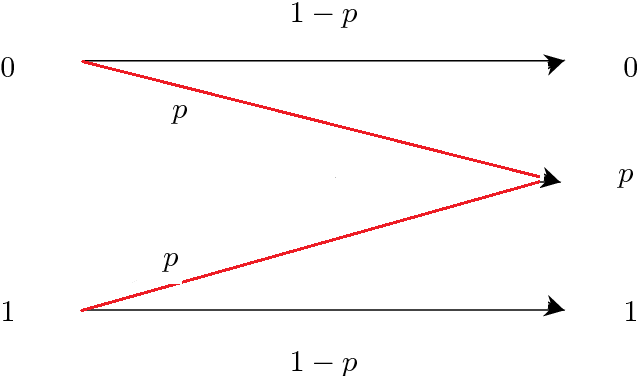
\includegraphics[width=0.5\linewidth]{img/avec_effacement.png}\\
\\
-Detecte au plus $\rho +1 \leq dm$ \\
-Corrige $2t+\rho +1 \leq dm$ \\
\\

\textbf{Code Parfait} : \\
Une condition necessaire est suffisante pour qu'un code lineaire $Ct$ correcteur et de distance minimum dm soit parfait : \\
$\sum\limits_{i=0}^t C_n^j(q-1)^j = q^k$\\
\\

\section{Generation et Detection}
La \textbf{matrice generatrice} est utiliser dans le cas des code lineaire ,exemple:\\
Avec n=4 et m=2 ou (n:nombre de mot , m:la longueur du mot)\\
On a g1=
\begin{pmatrix}
1 \\
0 \\
0 \\
0
\end{pmatrix}
et g2 =
\begin{pmatrix}
0 \\
1 \\
0 \\
0
\end{pmatrix}
\\
\\
\\
U=
\begin{bmatrix}
1 & 0 \\
0 & 1 \\
0 & 0 \\
0 & 0 
\end{bmatrix}
$\times$
\begin{pmatrix}
x \\
y \\
\end{pmatrix}\\
\\
Le mot a coder est de longueur 2 : 00,01,10,11\\
On vas ensuite prendre chaque mot et effectuer le produit matriciel par U:\\
\\
\begin{bmatrix}
1 & 0 \\
0 & 1 \\
0 & 0 \\
0 & 0 
\end{bmatrix}
$\times$
\begin{bmatrix}
1 \\
0 
\end{bmatrix}
=
\begin{bmatrix}
1 \\
0 \\
0 \\
0  
\end{bmatrix}\\
\\
Ducoup le mode coder est : 0000 , 0100 , 1000 ,1100\\
On peux ecrire le poid $dm$ (nb de 1) de chaque mot coder : 0 , 1 , 1 ,2 ici dm=1 (poid le plus faible)\\
On a donc dm-1 = 0 Detection\\
Et $\frac{dm-1}{2}$ Correction\\
\\
Un code lineaire systematique peux etre representer sous forme d'un systeme (m:message):\\
c1 = m1\\
c2 = m2\\
$- - - - - - -$\\
c3 = m1+m2\\
c4 = m1\\
c5 = m1+m2\\
\\
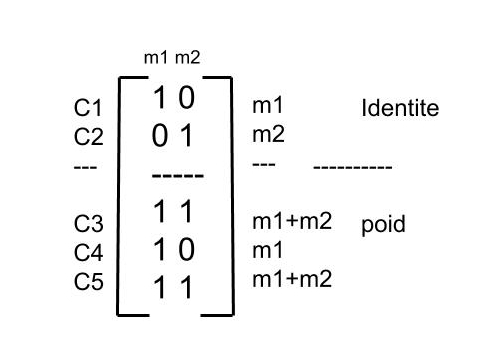
\includegraphics[width=0.5\linewidth,center]{img/matrice_generatrice.jpg}
\\
Selon le systeme du dessus on peux representer la matrice generatrice de cette facons :\\
G = \\
\\
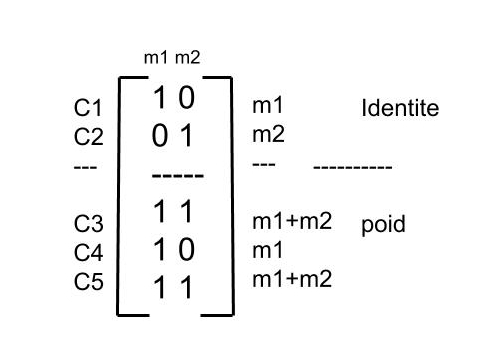
\includegraphics[width=0.2\linewidth,right]{img/matrice_generatrice.jpg}
\\
\textbf{Matrice de controle} :\\
Elle se note : 
H = 
\begin{bmatrix}
-P^T \\
I
\end{bmatrix}
\Rightarrow H^T =
\begin{bmatrix}
P \\
I
\end{bmatrix}
=
\begin{bmatrix}
1 & 1 & \| & 1 & 0 & 0 \\
1 & 0 & \| & 0 & 1 & 0 \\
1 & 1 & \| & 0 & 0 & 1
\end{bmatrix}\\
\\
$G^TH=0$\\
\\
\textbf{Syndrome} :\\
$C$ est un mot cod\'e , alors $H^TC=0$\\
$y$ est un mot recu , syndrome de $y$ : $s(y)=H^Ty$\\
$y=C+e$ avec e:erreur [0010] (on met un 1 sur le bit errone)\\ 
Donc $s(y)=s(C+e)=H^TC+H^Te=H^Te$\\
\\
\underline{Procedure} :\\
-Calculer $s(y)=H^Ty$ \\
-Si $s(y)=0$ alors y est le mot code\\
-Sinon on cherche une sequence $Z$ de longueur $n$ telle que $H^TZ=s(y)$ , $C=y+Z$\\

\section{Sequence d'hadamard}
Elle se definit comme suit et est de taille minimal 8 : 
\begin{bmatrix}
H & H \\
H & -H \\
\end{bmatrix}\\
\\
On commence a H0=
\begin{bmatrix}
1
\end{bmatrix}\\
H1 = 
\begin{bmatrix}
\begin{bmatrix}
1
\end{bmatrix} & 1 \\
1 & -1 
\end{bmatrix}\\
\\
\\
H2 =
\begin{bmatrix}
  \begin{bmatrix}
  1 & 1 \\
  1 & -1
  \end{bmatrix}
  &
  \begin{bmatrix}
  1 & 1 \\
  1 & -1
  \end{bmatrix}
  \\
  \begin{bmatrix}
  1 & 1 \\
  1 & -1
  \end{bmatrix}
  &
  \begin{bmatrix}
  -1 & -1 \\
  -1 & 1
  \end{bmatrix}
\end{bmatrix}\\
\\
\\
H3 =
\begin{bmatrix}
  \begin{bmatrix}
  1 & 1 & 1 & 1 \\
  1 & -1 & 1 & -1 \\
  1 & 1 & -1 & -1 \\
  1 & -1 & -1 & 1 
  \end{bmatrix}
  &
  \begin{bmatrix}
  1 & 1 & 1 & 1 \\
  1 & -1 & 1 & -1 \\
  1 & 1 & -1 & -1 \\
  1 & -1 & -1 & 1 
  \end{bmatrix}
  \\
  \begin{bmatrix}
  1 & 1 & 1 & 1 \\
  1 & -1 & 1 & -1 \\
  1 & 1 & -1 & -1 \\
  1 & -1 & -1 & 1 
  \end{bmatrix}
  &
  \begin{bmatrix}
  -1 & -1 & -1 & -1 \\
  -1 & 1 & -1 & 1 \\
  -1 & -1 & 1 & 1 \\
  -1 & 1 & 1 & -1 
  \end{bmatrix}
\end{bmatrix}\\
\\
Chaque ligne de la matrice correspond a une sequence , il y en a donc 8 par defaut .\\
Si un utilisateur U1 veux transmettre la sequence S1 "101" en utilisant la sequence 2 (2ieme ligne de la matrice) , on auras donc :\\
S1 : "1" seras code par la 2ieme lignes donc "1 -1 1 -1 1 -1 1 -1" et "0" par son inverse "-1 1 -1 1 -1 1 -1 1" \\
S1 = "101" \Rightarrow "1 -1 1 -1 1 -1 1 -1" "-1 1 -1 1 -1 1 -1 1" "1 -1 1 -1 1 -1 1 -1"\\
\\
Si U2 veux transmettre "011" on lui attribueras la sequence 4 par exemple (4ieme ligne de H) , on auras donc :\\
S2 = "011" \Rightarrow  "-1 1 1 -1 -1 1 1 -1" "1 -1 -1 1 1 -1 -1 1" "1 -1 -1 1 1 -1 -1 1" \\
\\
Maintenant si U1 et U2 veulent emettre en meme temps , il faudra faire une operation d'etalement S :\\
S=S1+S2\\
S="0 0 2 -2 0 0 2 -2" "0 0 -2 2 0 0" "2 -2 0 0 2 -2 0 0" 
%%%%%%%%%%%%%%%%%%%%%%%%%%%%%%%%%%%%%%%%%%%%%%%%%%%%%%%%%%%%%%%%%%%%%%%%%%%%%%
\chapter{Code Cyclique/ Pseudo-Aleatoire}

\section{Code Pseudo Aleatoire}

Un nombre n'etant pas al\'eatoire , on vas piocher une partie d'une tres grande sequence binaire .Cette sous-sequence seras genere de tel sorte qu'il ne seras presque impossible de trouver la meme sous-sequence.\\
La Sequence doit etre : \\
1) Generer facilement (seq. binaire 0,1)\\
2)Suffisament longue\\
3)Difficilement reconstituable par petit segment\\
4)Distribution des eb qui apparait de facons aleatoire (evite les meme suite de 0 et 1 ex: 001 01 001 1 001 001)\\
\\
\underline{Solution} : utiliser code a longueur maximal (LM) , code Gold ou JPL.\\

\subsection{Code a Longueur Maximal LM}
La fonction c , rand() utilise un code LM.\\
\\
\underline{Principe} : Il s'agit de registre a decalage en reaction lineaire composant n etages.\\
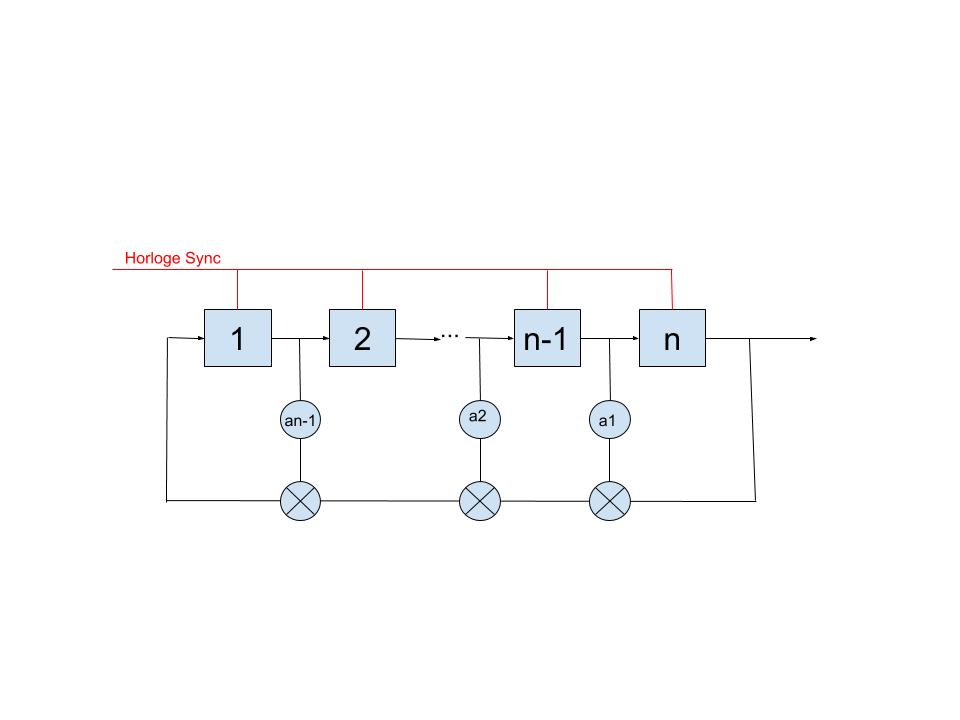
\includegraphics[width=0.75\linewidth,center]{img/code_LM.jpg}\\
\\
Le schema peux representer un polynome de second degre , ce systeme permet d'avoir autant de 0 que de 1 (Distributivite) , $L=(2^n-1)$ bits (L:taille)\\
\\
L'addition mod(\%) 2 d'une sequence LM avec une sequence d\'ecaler/repliqu\'e sur elle meme donne \Rightarrow une sequence LM repliqu\'e\\

\subsection{Code Gold}
Implemente le code LM mais permet de generer des sequence encore plus longue . Utilise dans le systeme CDMA (AMRC en anglais).\\
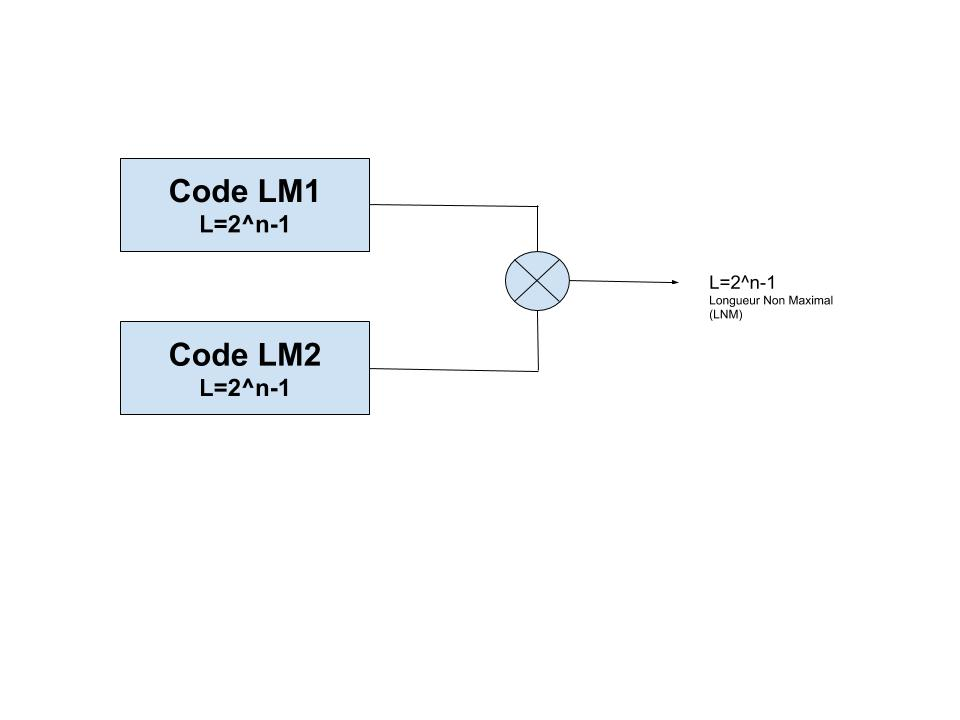
\includegraphics[width=0.75\linewidth,center]{img/code_Gold.jpg}\\
\\
Inutile si on prend 2 fois le meme sequence car LM1 et LM2 sont demarrer et initialiser en meme temps .\\
\\
\underline{Exemple} : \textbf{Registre a decalage} de longueur 4\\
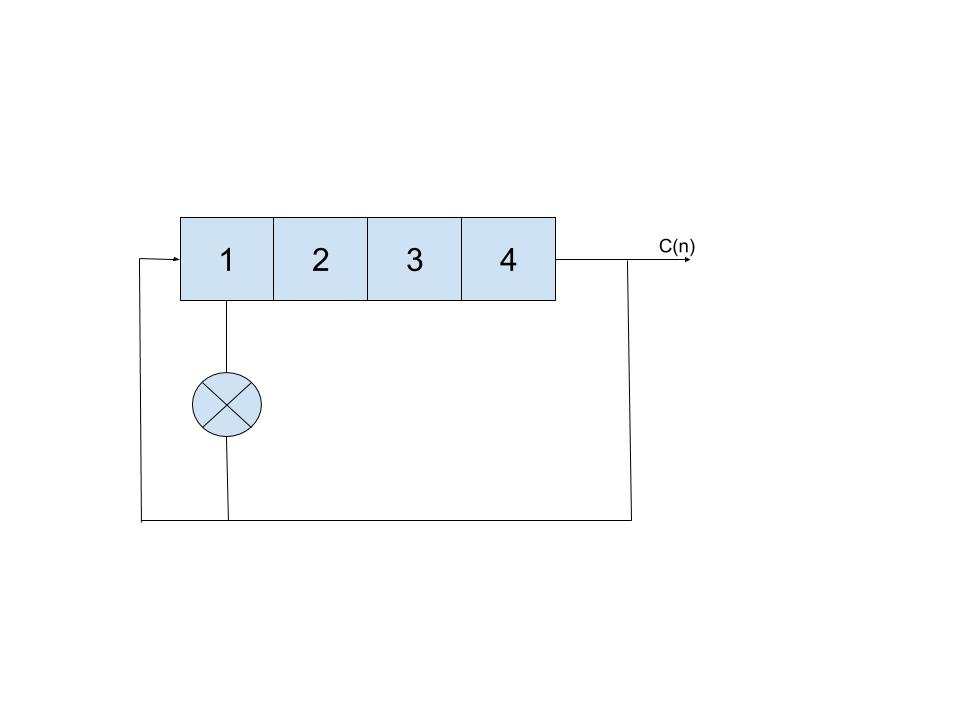
\includegraphics[width=0.75\linewidth,center]{img/registre_a_decalage.jpg}\\
On preleve sur le 1er et 4ieme element [4,1].\\
\\
-Initialisation : cela peux etre fait avec des valeurs quelconque $\diff$ de la sequence "0000" , en generale on initialise a "1111".\\
\\
\underline{Principe} : \\
1)Decalage de la sequence de 1 rang vers la droite\\
2)Xor [4,1] : On fait un ou-exclusif sur le 1er et le 4ieme element jusqu'a  temps de retomber sur la sequence initial "1111"\\
\\
\begin{matrix}
Cn     & 1 & 1 & 1& 1 \\
C(n+1) & 0 & 1 & 1& 1 \\
C(n+2) & 1 & 0 & 1& 1 \\
C(n+3) & 0 & 1 & 0& 1 \\
C(n+4) & 1 & 0 & 1& 0 \\
C(n+5) & 1 & 1 & 0& 1 \\
       &   &   &  &   \\
C(n+6) & 0 & 1 & 1& 0 \\
C(n+7) & 0 & 0 & 1& 1 \\
C(n+8) & 1 & 0 & 0& 1 \\
C(n+9) & 0 & 1 & 0& 0 \\
C(n+10) & 0 & 0 & 1& 0 \\
C(n+11) & 0 & 0 & 0& 1 \\
C(n+12) & 1 & 0 & 0& 0 \\
C(n+13) & 1 & 1 & 0& 0 \\
C(n+14) & 1 & 1 & 1& 0 \\
C(n+15) & 1 & 1 & 1& 1 
\end{matrix}\\
\\
$L=2^n-1=15 (on prend pas la 1er ligne d'initialisation$\\
\\
La lecture des Cn se lis en colonne , Cn commenceras donc par la premier ligne et C(n+6) respectivement a la 6ieme lignes d'ou l'espacement de le systeme, ce qui donne :\\
\\
C(n)   : 1111 0101 100 1000\\
C(n+6) : 0110 0100 011 1101\\ 
C(n) xor C(n+6) = 1001 0001 111 0101\\
\\
\underline{Propriete} : 
-Il n'y a aucune serie de "0" de longueur R\\
-Il y a qu'une serie de "1" de longueur R\\
-Il y a qu'une serie de "0" de longueur R-1\\
-Il n'y a aucune serie de "1" de longueur R-1\\
-Il y a  $2^{R-P-2}$ serie de "0" de longueur P\\
-Il y a $2^{R-P-2}$ serie de "1" de longueur P\\
\\
Si on prend :\\
R=4 : On a 0 serie de "0000" et 1 serie de "1111" (rouge)\\
R-1=3 : On a 1 serie de "000" et 0 serie de "111" (vert)\\
P=2 : On a $2^{4-2-2}=2^0=1$ donc 1 serie de "00" et 1 serie de "11" (orange)\\
P=1 : On a $2^{4-1-2}=2^1=2$ donc 2 serie de "0" et 2 serie de "1" (bleue)\\
\\
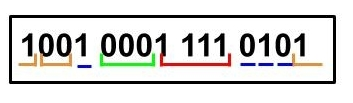
\includegraphics[width=0.5\linewidth,center]{img/registre_decalage_exemple.jpg}\\
\\

\underline{Note} : Pour avoir les meilleur resultat , des chercheurs ont trouve un polynome qui possede assez de combinaisons pour etre dit fiable , on parle du polynome 89 [89,6,5,3]\\




\subsection{Code JPL}
Implementation de plusieur code LM avec une taille differente (n\diff m\diff p) , ce systeme est utilis\'e en radio-localistion (GPS).\\
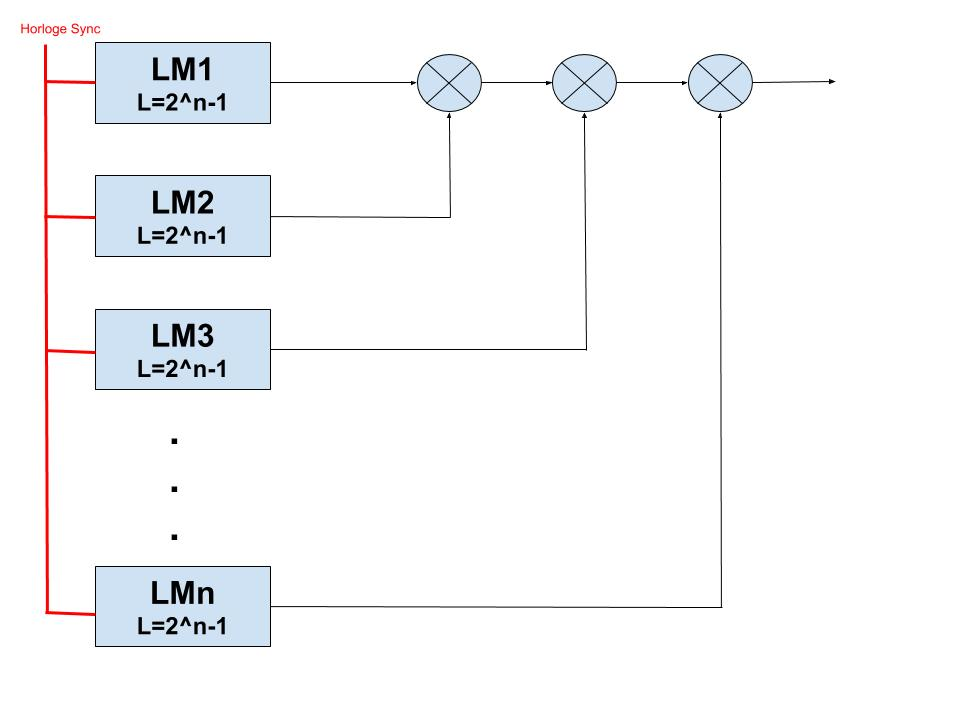
\includegraphics[width=0.75\linewidth,center]{img/code_JPL.jpg}\\
\\
LM1,LM2 et LM3 doivent etre premier entre eux .\\
\\


\section{Code Cyclique}
Code le plus utilise dans de nombreux systeme.Les code cyclique sont detecteur et correcteur d'erreur .Les bits de controle sont le reste de la division polynomial.\\
\\
\underline{Exemple} : \\
Determinez si le code engendre par la matrice est cyclique ?
Avec G=
\begin{bmatrx}
1 & 1 & 0 & 0 \\
0 & 1 & 1 & 0 \\
0 & 0 & 1 & 1  
\end{bmatrx}\\
\\
On vas effectuer le produit matriciel avec une matrice M \\
M=
\begin{bmatrx}
0 & 0 & 0  \\
0 & 0 & 1  \\
0 & 1 & 0  \\  
0 & 1 & 1  \\
1 & 0 & 0  \\
1 & 0 & 1  \\
1 & 1 & 0  \\
1 & 1 & 1  
\end{bmatrx}\\
\\
On a donc $M\times G=C$\\
C=
\begin{bmatrx}
0 & 0 & 0 & 0 \\
0 & 0 & 1 & 1 \\
0 & 1 & 1 & 0 \\
0 & 1 & 0 & 1 \\
1 & 1 & 0 & 0 \\
1 & 1 & 1 & 1 \\  
1 & 0 & 1 & 0 \\ 
1 & 0 & 0 & 1  
\end{bmatrx}\\
\\
Si on decale une ligne sur la gauche on retombe sur une autre ligne de la matrice , C est cyclique si tout les lignes sont decalable\\

%%%%%%%%%%%%%%%%%%%%%%%%%%%%%%%%%%%%%%%%%%%%%%%%%%%%%%%%%%%%%%%%%%%%%%%%%%%%%%
\chapter{Temps Reel}

\end{document}